% begin module 
\begin{frame}
\frametitle{The Disk Method}
 {\it{To find the volume of a solid of revolution using the disk method, use one of the following:}} \\

\begin{center}
{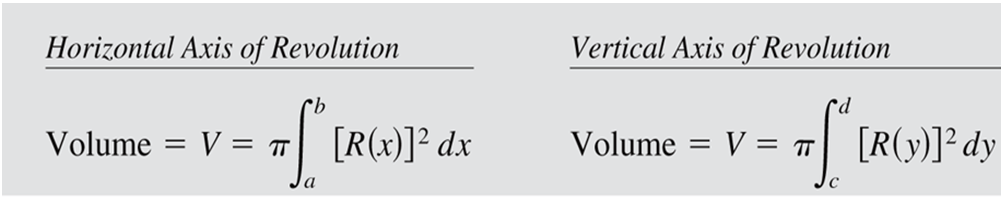
\includegraphics[width=.7\textwidth]{volumes/pictures/Disk1}}
\end{center}


\begin{center}
{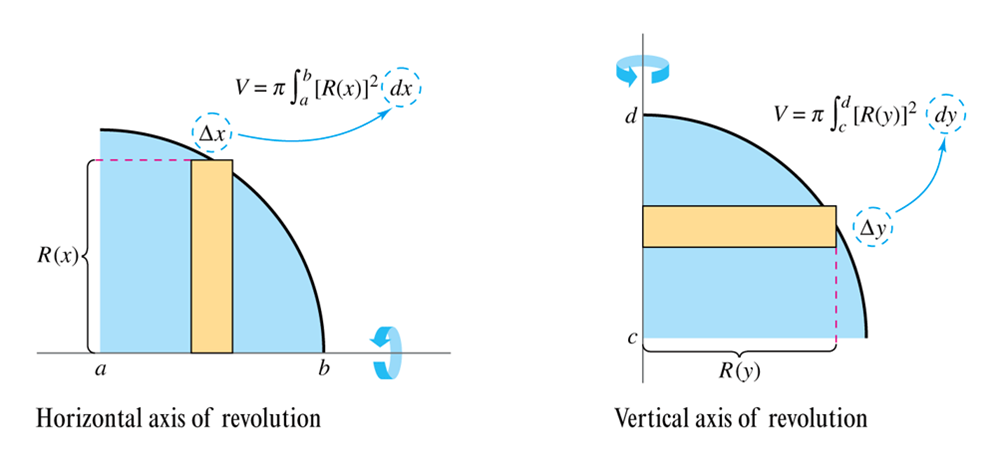
\includegraphics[width=.8\textwidth]{volumes/pictures/Disk2}}
\end{center}


\end{frame}


\begin{frame}
\begin{example}[Vertical axis of rotation]
The region between the curves $ \ds x=\frac{1}{\sqrt{y}} $, $ y=1$, $y=4  $, and the $y$-axis is revolved about the $y$-axis. Find the volume.
\begin{columns}[c]
\column{.5\textwidth}
\uncover<2->{
Solution:\\ 
We use a horizontal disk (perpendicular to the axis of rotation).
 The thickness is $dy$} %
\uncover<3->{
The radius is the $x$ value of the function, $ x=\frac{1}{\sqrt{y}} $ } %
\column{.5\textwidth}
\uncover<1>{
{\includegraphics<1>[width=.4\textwidth]{volumes/pictures/vol1}}
} %
\uncover<2->{
{\includegraphics<2->[width=.5\textwidth]{volumes/pictures/vol1b}}
}
\end{columns}

\uncover<4->{ Therefore, we have}     
\[
\uncover<4->{V=\int_{1}^4  \pi\left( \frac{1}{\sqrt{y}} \right)^2\;dy}\uncover<5->{=\int_{1}^4  \pi \frac{1}{y} \;dy} \uncover<6->{= \pi\cdot \left.\ln|y|\right|_{1}^4} 
\]
\[
\uncover<7->{= \pi\ln(4)-\pi\ln(1)} \uncover<8->{ = \pi \ln(4).}
\]
 %{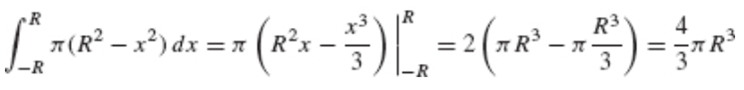
\includegraphics[width=\textwidth]{volumes/pictures/v3}}
\end{example}
\end{frame}



